\chapter{Thermal Expansion}
\label{ch:thermalExpansion}

\section{Necessity of Modeling}
  The fast reactor is entirely composed of metals and, as such,
  experiences significant thermal expansion. While other designs may employ
  non-metallic fuel material (e.g. oxides or carbides), these are not considered
  in this work. Reactor designs with metal fuel include \gls{ebr-ii}, as
  designed and built by \gls{anl}, and PRISM, as designed by \gls{geh}.

  In metal fueled reactors, thermal expansion represents a significant
  reactivity feedback effect.  The preliminary safety information document for
  PRISM presents an estimate for thermal expansion feedback such that a 1\%
  increase in radial dimension results in $-0.5 \units{$\Delta k$}$ indicating a
  significant effect \cite{GEFR793}. Additionally, thermal expansion has been
  demonstrated to serve as an inherent safety feature of fast reactors. In the
  remarkable \gls{ebr-ii} demonstrations in April 1986, two major accident
  demonstrations were performed on the reactor while operating at full power.
  Operators forced the reactor to undergo \gls{ulof} and \gls{ulohs} events.
  \gls{ebr-ii} was safely shutdown due to nothing other than inherent
  multiphysics feedback effects. These experiments demonstrated conclusively the
  passive safety of fast reactor designs, due in part to the thermal expansion
  of materials \cite{PlentifulEnergy}.

  \gls{ebr-ii} system response to \gls{ulof} was demonstrated by bypassing the
  normal loss of flow scram (i.e. shutdown) function. The control rod drive
  motors were deenergized and the main coolant pumps were tripped off and
  allowed to coast down. Natural circulation flow followed and, after an initial
  temperature peak, material temperatures returned to normal operating
  temperatures \cite{ebriitests}. 
  
  The \gls{ulohs} response was demonstrated by
  shutting down coolant pumps in the secondary coolant system, thereby disabling
  heat rejection from the primary coolant system. No subsequent automatic or
  manual action was taken. In the \gls{ulohs} demonstration, material
  temperatures did not peak and instead quickly reduce below operating
  temperatures \cite{ebriitests}.

  The inherent safety demonstration test at \gls{ebr-ii} demonstrated the
  passive safety of the liquid metal cooled and metal fueled reactor design.
  These tests are simply not possible with currently operating \glspl{lwr}
  designs. Using nothing but natural phenomena, the reactor was demonstrated to
  shutdown and subsequent heat removal was achieved \cite{ebriitests}. These
  tests are pivotal the strategy to demonstrate the performance of similar
  reactors in \gls{atws} events. The tests also demonstrate the importance of 
  modeling multiphysics effects in fast reactor applications.

\section{Material Properties}
  \label{sec:model_details__material_properties}
  All structural materials in the reactor are thermally expanded as HT9
  stainless steel. Fuel material is thermally expanded as metallic uranium
  with 10\% Zr by weight included (i.e. U10Zr). The equations for the
  \gls{lef} used in this work are given as functions of temperature
  \begin{equation}
    \label{eq:lef_ht9}
    \left( \frac{\Delta L}{L} \right)_{\text{HT9}} = 
      -2.191 \times 10^{-3} + 5.678 \times 10^{-6} \, T + 
      8.111 \times 10^{-9} \, T^2 - 2.576 \times 10^{-12} \, T^3 ,
      % zero at 282.26 [K], 48.398 [degF]
  \end{equation}
  \begin{multline}
    \label{eq:lef_u10zr}
    \left( \frac{\Delta L}{L} \right)_{\text{U10Zr}} = \\
      \begin{cases}
        -7.3 \times 10^{-3} + 3.489 \times 10^{-5} \, T 
          - 5.154 \times 10^{-8} \, T^2 + 4.39 \times 10^{-11} \, T^3 & 
          T \le 923 \units{K}, \\
        -0.25252 + 6.669 \times 10^{-4} \, T - 5.441 \times 10^{-7} \, T^2 
          + 1.518 \times 10^{-10} \, T^3 & \text{otherwise},
      \end{cases}
      % zero at 318.34 [K], 113.34 [degF]
  \end{multline}
  for $T$ in \units{K} \cite{ht9Prop,thexpU10Zr}. Note that U10Zr undergoes a
  phase change at $923 \units{K}$ that increases the \gls{lef} at this point.
  Both \eref{eq:lef_ht9} and \eref{eq:lef_u10zr} evaluate to zero near room
  temperature. The \gls{lef} of HT9 and U10Zr over the range of operating
  temperatures of fast reactors are plotted in \fref{fig:lef_plot}. It is
  observed that the \gls{lef} of U10Zr is as much as twice that of HT9. This
  implies fuel material will expand significantly more than structural
  material.

  \begin{figure}
    \centering
    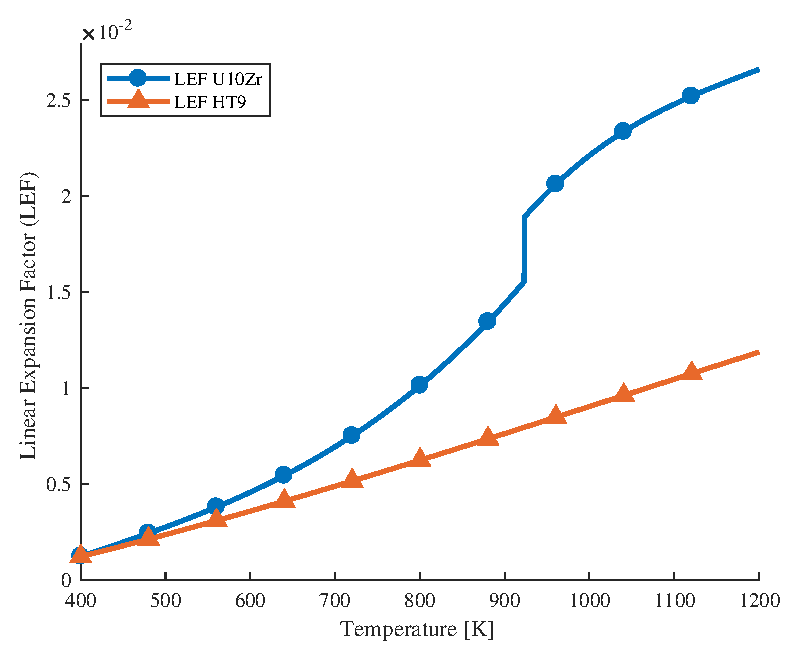
\includegraphics[width=0.7\textwidth]{lef_plot}
    \caption{Linear Expansion Factor for HT9 Steel and U10Zr Fuel.}
    \label{fig:lef_plot}
  \end{figure}

  All sodium in the reactor is assumed to be liquid.  Therefore, effects of
  thermal expansion within sodium are described by the change in density as a
  function of temperature \cite{sodiumProp}, not by an \glsentryshort{lef}. 
  Consistent with this assumption, the mass of sodium within the reactor is not
  conserved. Sodium coolant will flow into and out of the reactor vessel as
  structural components thermally expand. Sodium in the bond region will flow
  upward within the cladding into a gas plenum at the top of the fuel rod as the
  fuel thermally expands. This is not modeled as the sodium level in the bond is
  not tracked.
    
\section{Model Details}
  \label{sec:model_details}
  Thermal expansion contributes two main categories of feedback effects: leakage
  effects and density effects. Increased reactor dimensions due to thermal
  expansion increases neutron leakage from the reactor. The neutron leakage
  fraction is the fraction of neutrons created in the fuel due to fission that
  exit the core. The leakage fraction can be expressed as
  \begin{equation}
    \label{eq:leakage}
    \leakage = \frac{\keff}{k_{\infty}}
  \end{equation}
  where $k_{\infty}$ is the effective neutron multiplication factor for an
  infinite medium. \glspl{lwr} typically have low and ultra-low leakage
  designs with $\leakage \approx 2 \%$ \cite{textbookknief}. However, fast
  reactors simulated in this work have $\leakage \approx 20\%$ and are
  therefore highly sensitive to changing reactor dimensions due to thermal 
  expansion.

  Density effects of thermal expansion are a consequence of the conservation of
  material within the reactor. As reactor dimensions expand, the reactor volume
  increases. However, the quantity of material in the reactor vessel remains 
  unchanged. Therefore, material densities must be decreased proportionally to
  the increase of reactor dimensions. Decreasing material densities results in
  decreased macroscopic neutron cross sections due to the proportionality
  $\Sigma = N \, \sigma$ where $\Sigma$ is a macroscopic cross section, $N$ is a
  number density, and $\sigma$ is a microscopic cross section.

  Highly detailed thermal expansion modeling can be performed using the
  \gls{fem} to calculate local stresses and strains on all reactor
  structural components such as fuel pins, wire wraps, and assembly cans.
  However, this would require a significantly more advanced model and improved
  spatial resolution. The model developed here for the simulation of fast
  reactors does not estimate temperature and heat generation at all positions
  due to the smearing of hexagonal assemblies. Therefore, a simplified thermal
  expansion model is developed.  This simplified model expands finite element
  coordinates uniformly throughout the reactor, expands area fractions within
  finite elements, and decreases number densities accordingly.

  All dimensions in the reactor are expanded assuming the user-input
  dimensions are at room-temperature conditions. Dimensions are expanded
  according to two user-input temperatures, \texpfuel and \texpstruct.
  \texpfuel corresponds to the average temperature of fuel material in the
  reactor and \texpstruct corresponds to the average temperature of structural
  material in the reactor. Typically, these values come from a previous
  coupled neutron diffusion and thermal hydraulics simulation. \texpfuel and
  \texpstruct must be known before a thermal expansion simulation begins. This
  is acceptable because the \glspl{lef} from \eref{eq:lef_ht9} and
  \eref{eq:lef_u10zr} are on the order $10^{-2}$ so small changes in
  user-input temperatures will be insignificant.

  \subsection{Expansion of Finite Element Coordinates}
    \label{sec:expansion_of_fe_coordinates}
    In the simplified thermal expansion model developed for this work, the
    coordinates of finite elements are expanded uniformly in the axial and
    radial directions. In the radial (both $x$ and $y$) directions,
    it is assumed that elements expand as structural material. Specifically,
    $x$ and $y$ coordinates are expanded using HT9 material properties from
    \eref{eq:lef_ht9}. The dominant effect on $\keff$ due to thermal expansion
    in the radial directions is the expansion of the hexagonal assemblies
    themselves and the expansion of the grid plate at the base of the reactor,
    all of which are composed of HT9 stainless steel. In the axial direction
    (the $z$ direction), it is assumed that elements expand as fuel material,
    U10Zr, using the \gls{lef} from \eref{eq:lef_u10zr}. The dominant effect on
    $\keff$ due to thermal expansion in the axial direction is the elongation of
    the metallic fuel.

    Assuming the uniform radial expansion of elements specified by
    \eref{eq:lef_ht9} and \texpstruct, a radial \gls{lef} can be defined as
    \begin{equation}
      \label{eq:lef_r}
      F_r(\texpstruct) = 1 + \left(\frac{\Delta L}{L}\right)_{\text{HT9}}
    \end{equation}
    which is a function of \texpstruct. Similarly, an axial \gls{lef} can be
    defined using \eref{eq:lef_u10zr} and \texpfuel.
    \begin{equation}
      \label{eq:lef_a}
      F_a(\texpfuel) = 1 + \left(\frac{\Delta L}{L}\right)_{\text{U10Zr}}
    \end{equation}
    This assumption of uniform expansion of elements in the radial and axial
    directions is depicted in \fref{fig:thexp_figure}. \fref{fig:thexp_figure}
    shows a general volume being thermally expanded in radial directions
    according to \eref{eq:lef_r} and the axial direction according to
    \eref{eq:lef_a}.

    \begin{figure}
      \centering
      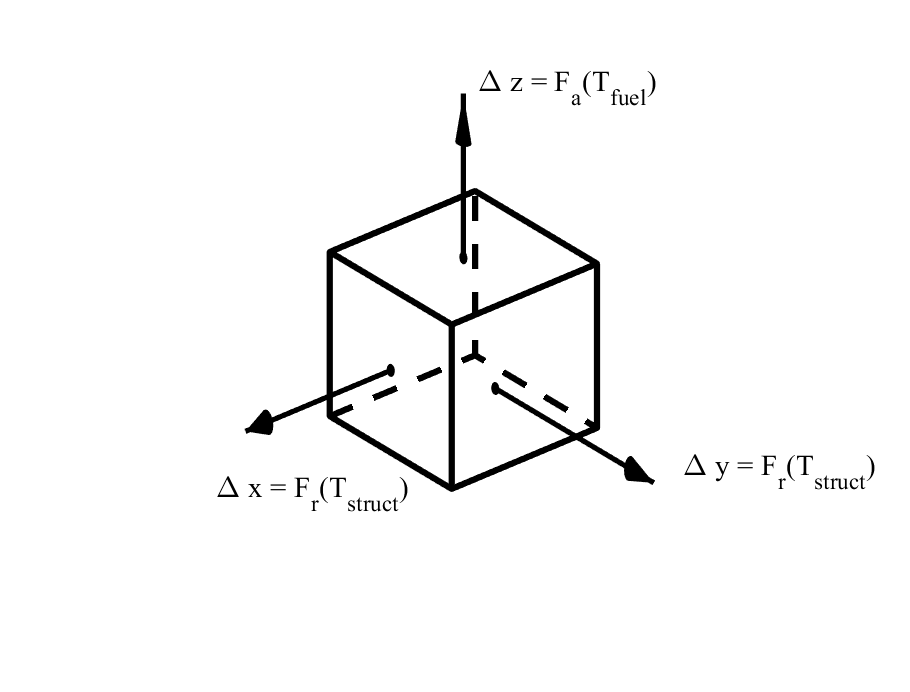
\includegraphics[width=0.7\textwidth]{thexp_figure}
      \caption{Thermal Expansion of General Volume.}
      \label{fig:thexp_figure}
    \end{figure}

    Since all elements are being expanded at the same rate, they will not
    intersect or overlap. Due to the uniform expansion of elements, the ``cold''
    coordinate $(x^C,y^C,z^C)$ can be thermally expanded to the ``hot''
    coordinate $(x^H,y^H,z^H)$ using \eref{eq:lef_r} and \eref{eq:lef_a}.
    \begin{align}
      \label{eq:expand_x}
      x^H &= x^C \, F_r(\texpstruct), \\
      \label{eq:expand_y}
      y^H &= y^C \, F_r(\texpstruct), \\
      \label{eq:expand_z}
      z^H &= z^C \, F_a(\texpfuel),
    \end{align}
    \eref{eq:expand_x}, \eref{eq:expand_y} and \eref{eq:expand_z} uniformly
    expand the distance from each coordinate to the origin. Thus, the coordinate
    thermal expansion equations are applied to each coordinate in the finite
    element mesh to uniformly expand all elements.

  \subsection{Expansion of Area Fractions}
    \label{sec:expansion_of_area_fractions}
    The thermal expansion of the dimensions of hexagonal assemblies themselves 
    has been modeled with the assumption of uniform expansion of finite elements
    in \sref{sec:expansion_of_fe_coordinates}. Dimensions within a hexagonal
    assembly, such as fuel radius, are expanded by modifying area fractions.
    These thermally expanded area fractions are then used to homogenize cross
    sections within an assembly as in \sref{sec:cross_section_treatment}.

    The radius of the fuel rod, $R_F$, is expanded using the \gls{lef} for
    U10Zr from \eref{eq:lef_u10zr}. All other dimensions within the hexagonal
    assembly (wire wrap diameter, can thickness, flat-to-flat measurement, etc.)
    are expanded using the \gls{lef} for HT9 from \eref{eq:lef_ht9}. Note that
    due to the magnitudes of these \glspl{lef}, it is possible for $R_F$ to
    exceed the inner radius of the cladding. This is a non-physical result and
    will only occur for small sodium bond gaps and high thermal expansion
    temperatures. In these cases, the radius of the fuel is confined to the
    thermally expanded inner radius of the cladding. Though a more complex
    relationship describes the true value of these radii, the resolution of this
    model does not allow for such detail.
    
    Thermally expanded area fractions are calculated by first thermally 
    expanding each dimension within a hexagonal assembly. Then, cross-sectional
    areas and resulting area fractions are calculated using the formulae from
    \sref{sec:geometry_description}. By using these formulae, the sodium bond
    and sodium coolant area fractions will be allowed to ``float.'' That is, the
    sodium area fraction will decrease appropriately to allow for the expansion
    of other materials within the assembly. Recall, the mass of sodium in the
    reactor is not conserved. Finally, the calculated areas are used to
    calculate area fractions and homogenize cross sections within a hexagonal
    assembly.
  
  \subsection{Conservation of Material and Cross Section Effects}
    \label{sec:cross_section_effects}
    After thermally expanding finite elements and area fractions within
    assemblies, material densities are decreased to conserve quantity of
    material in the reactor. In this derivation, the conservation of reactor 
    material is expressed as a conservation of number of atoms. The conservation 
    of the number of atoms for species $i$, can be expressed as
    \begin{equation}
      \label{eq:conservation}
      n_i^H = n_i^C 
    \end{equation}
    where $n_i^H$ is the number of atoms of species $i$ after thermal expansion,
    i.e. ``hot,'' 
    and $n_i^C$ is the number of atoms of species $i$ before thermal expansion,
    i.e. ``cold.'' The number of atoms $n_i$ can be written as 
    \begin{equation}
      \label{eq:nden_definition}
      n_i = N_i \, V_i
    \end{equation}
    where $N_i$ is the number density of species $i$ and $V_i$ is the volume
    occupied by species $i$. Then, inserting \eref{eq:nden_definition} into 
    \eref{eq:conservation} yields an expression for the thermally expanded 
    number density of species $i$ as
    \begin{align}
      N_i^H \, V_i^H &= N_i^C \, V_i^C, \\
      \label{eq:nden_volume_ratio}
      N_i^H &= N_i^C \frac{V_i^C}{V_i^H},
    \end{align}
    where the term $\frac{V_i^C}{V_i^H} < 1$ and represents the expansion of the
    volume occupied by species $i$. 

    The volume $V_i$ can be written in terms of element volume and area
    fraction. Let species $i$ be contained in region $j$ in finite element $e$. 
    This work assumes area fractions are constant within an element and can be
    treated as volume fractions. Then, the volume $V_i$ can be rewritten as 
    $V_i = a_j \, V_e$ where $a_j$ is the area fraction of region $j$ and $V_e$
    is the volume of element $e$. Inserting this definition for $V_i$ into
    \eref{eq:nden_volume_ratio}.
    \begin{equation}
      \label{eq:nden_expansion_expanded}
      N_i^H = N_i^C \frac{a_j^C \, V_e^C}{a_j^H \, V_e^H}
    \end{equation}
    The ratio of area fractions, $\frac{a_j^C}{a_j^H}$, is calculate directly
    using cold and hot area fractions as described in
    \sref{sec:expansion_of_area_fractions}. The ratio of element volumes
    $\frac{V_e^C}{V_e^H}$ can be rewritten using the relationships
    \eref{eq:lef_r} and \eref{eq:lef_a}.

    Begin by considering a volume such as \fref{fig:thexp_figure}. Define the
    volume $V^C = L_x^C \, L_y^C \, L_z^C$ with $L_x^C$, $L_y^C$, and $L_z^C$
    representing the ``cold'' lengths of the volume. The thermally expanded
    volume, $V^H$, can then be written
    \begin{equation}
      V^H = (L_x^C + \Delta L_x) (L_y^C + \Delta L_y) (L_z^C + \Delta L_z).
    \end{equation}
    Recognizing the expansion of coordinates from \eref{eq:expand_x},
    \eref{eq:expand_y}, and \eref{eq:expand_z}.
    \begin{align}
      V^H &= (L_x^C \, F_r(\texpstruct)) (L_y^C \, F_r(\texpstruct)) 
        (L_x^C \, F_a(\texpfuel)) \\
      V^H &= L_x^C \, L_y^C \, L_z^C \,(F_r(\texpstruct))^2 \,
        F_a(\texpfuel) \\
      V^H &= V^C \, (F_r(\texpstruct))^2 \, F_a(\texpfuel) 
    \end{align}
    The element volume expansion ratio is then
    \begin{equation}
      \label{eq:volume_ratio}
      \frac{V^C}{V^H} = \frac{1}{(F_r(\texpstruct))^2 F_a(\texpfuel)}.
    \end{equation}
    \eref{eq:volume_ratio} can now be substituted into
    \eref{eq:nden_expansion_expanded}.
    \begin{equation}
      \label{eq:nden_thexp_update}
      N_i^H = N_i^C \frac{a_j^C}{a_j^H} 
        \frac{1}{(F_r(\texpstruct))^2 (F_a(\texpfuel))}
    \end{equation}
    To preserve the number of atoms in the reactor, material number densities
    must be updated according to \eref{eq:nden_thexp_update} in addition to
    expanding element coordinates and area fractions. Notice that
    \eref{eq:nden_thexp_update} can also be used to directly update neutron
    cross sections directly as they are proportional to number density.
    
\section{Results}
  The effect of thermal expansion on the effective neutron multiplication
  factor, $\keff$, is shown in this section. As stated previously in
  \sref{sec:model_details}, the user must input effective temperatures to which
  the reactor is thermally expanded. These user-input values, $\texpfuel$ and
  $\texpstruct$, are varied and all other thermal feedback effects are disabled
  in the simulation. For this simplified demonstration, $\texpfuel=\texpstruct$.
  It is expected that thermal expansion will cause a significant decrease in
  $\keff$ and represent negative reactivity insertion. Effective neutron
  multiplication factor as a function of thermal expansion is plotted in
  \fref{fig:thexp_study} and the associated reactivity, calculated as
  \begin{equation}
    \label{eq:reactivity_formula}
    \Delta \rho \units{\glsentryshort{pcm}} = 
      \frac{\keff - \kref}{\keff \, \kref} \times 10^5
  \end{equation}
  is plotted in \fref{fig:thexp_study_reactivity}. In
  \eref{eq:reactivity_formula}, $\keff$ is the calculated effective neutron
  multiplication factor after thermal expansion and $\kref$ is the neutron
  multiplication factor without thermal expansion. 

  Given the assumptions in this model, \fref{fig:thexp_study} and
  \fref{fig:thexp_study_reactivity} show that thermal expansion represents a
  significant reactivity effect and contributes as much as $-1,000
  \units{\glsentryshort{pcm}}$ at extreme temperatures. Additionally, in this
  model the thermal expansion factor of the fuel given in \eref{eq:lef_u10zr}
  dominates and the phase change given by the formula can be seen at the
  expected $923 \units{K}$.

  In the next chapter, the results of thermal expansion, along with thermal
  hydraulic feedback will be shown for a real reactor application.

  \begin{figure}
    \centering
    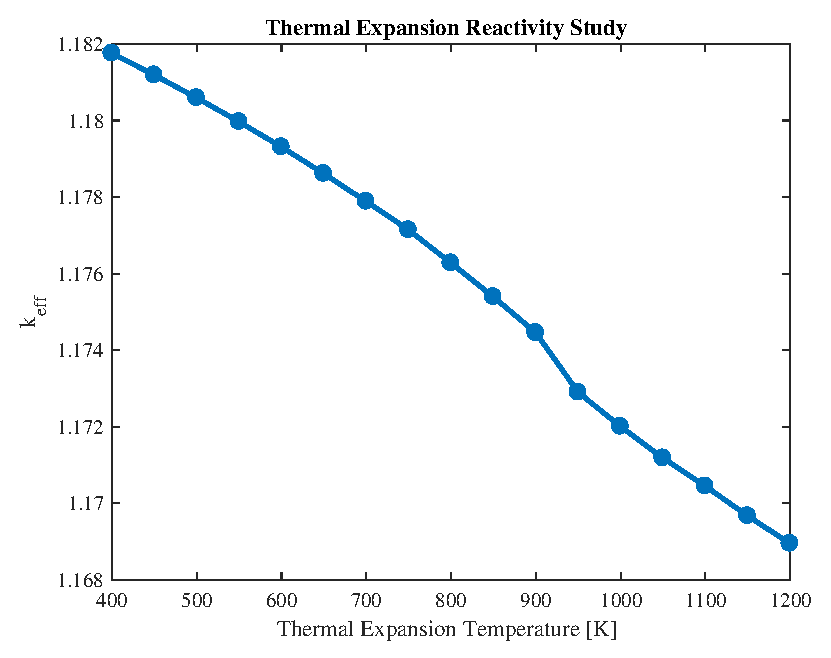
\includegraphics[width=0.7\textwidth]{thexp_study}
    \caption{Effective Neutron Multiplication Factor as a Function of 
      Thermal Expansion Temperature.}
    \label{fig:thexp_study}
  \end{figure}

  \begin{figure}
    \centering
    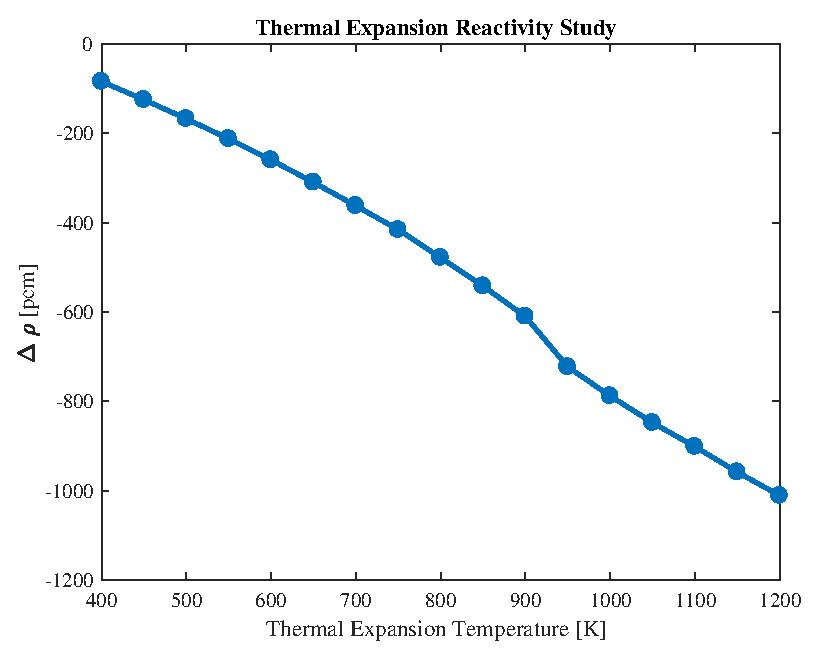
\includegraphics[width=0.7\textwidth]{thexp_study_reactivity}
    \caption{Reactivity as a Function of Thermal Expansion Temperature.}
    \label{fig:thexp_study_reactivity}
  \end{figure}
